\documentclass[1p]{elsarticle_modified}
%\bibliographystyle{elsarticle-num}

%\usepackage[colorlinks]{hyperref}
%\usepackage{abbrmath_seonhwa} %\Abb, \Ascr, \Acal ,\Abf, \Afrak
\usepackage{amsfonts}
\usepackage{amssymb}
\usepackage{amsmath}
\usepackage{amsthm}
\usepackage{scalefnt}
\usepackage{amsbsy}
\usepackage{kotex}
\usepackage{caption}
\usepackage{subfig}
\usepackage{color}
\usepackage{graphicx}
\usepackage{xcolor} %% white, black, red, green, blue, cyan, magenta, yellow
\usepackage{float}
\usepackage{setspace}
\usepackage{hyperref}

\usepackage{tikz}
\usetikzlibrary{arrows}

\usepackage{multirow}
\usepackage{array} % fixed length table
\usepackage{hhline}

%%%%%%%%%%%%%%%%%%%%%
\makeatletter
\renewcommand*\env@matrix[1][\arraystretch]{%
	\edef\arraystretch{#1}%
	\hskip -\arraycolsep
	\let\@ifnextchar\new@ifnextchar
	\array{*\c@MaxMatrixCols c}}
\makeatother %https://tex.stackexchange.com/questions/14071/how-can-i-increase-the-line-spacing-in-a-matrix
%%%%%%%%%%%%%%%

\usepackage[normalem]{ulem}

\newcommand{\msout}[1]{\ifmmode\text{\sout{\ensuremath{#1}}}\else\sout{#1}\fi}
%SOURCE: \msout is \stkout macro in https://tex.stackexchange.com/questions/20609/strikeout-in-math-mode

\newcommand{\cancel}[1]{
	\ifmmode
	{\color{red}\msout{#1}}
	\else
	{\color{red}\sout{#1}}
	\fi
}

\newcommand{\add}[1]{
	{\color{blue}\uwave{#1}}
}

\newcommand{\replace}[2]{
	\ifmmode
	{\color{red}\msout{#1}}{\color{blue}\uwave{#2}}
	\else
	{\color{red}\sout{#1}}{\color{blue}\uwave{#2}}
	\fi
}

\newcommand{\Sol}{\mathcal{S}} %segment
\newcommand{\D}{D} %diagram
\newcommand{\A}{\mathcal{A}} %arc


%%%%%%%%%%%%%%%%%%%%%%%%%%%%%5 test

\def\sl{\operatorname{\textup{SL}}(2,\Cbb)}
\def\psl{\operatorname{\textup{PSL}}(2,\Cbb)}
\def\quan{\mkern 1mu \triangleright \mkern 1mu}

\theoremstyle{definition}
\newtheorem{thm}{Theorem}[section]
\newtheorem{prop}[thm]{Proposition}
\newtheorem{lem}[thm]{Lemma}
\newtheorem{ques}[thm]{Question}
\newtheorem{cor}[thm]{Corollary}
\newtheorem{defn}[thm]{Definition}
\newtheorem{exam}[thm]{Example}
\newtheorem{rmk}[thm]{Remark}
\newtheorem{alg}[thm]{Algorithm}

\newcommand{\I}{\sqrt{-1}}
\begin{document}

%\begin{frontmatter}
%
%\title{Boundary parabolic representations of knots up to 8 crossings}
%
%%% Group authors per affiliation:
%\author{Yunhi Cho} 
%\address{Department of Mathematics, University of Seoul, Seoul, Korea}
%\ead{yhcho@uos.ac.kr}
%
%
%\author{Seonhwa Kim} %\fnref{s_kim}}
%\address{Center for Geometry and Physics, Institute for Basic Science, Pohang, 37673, Korea}
%\ead{ryeona17@ibs.re.kr}
%
%\author{Hyuk Kim}
%\address{Department of Mathematical Sciences, Seoul National University, Seoul 08826, Korea}
%\ead{hyukkim@snu.ac.kr}
%
%\author{Seokbeom Yoon}
%\address{Department of Mathematical Sciences, Seoul National University, Seoul, 08826,  Korea}
%\ead{sbyoon15@snu.ac.kr}
%
%\begin{abstract}
%We find all boundary parabolic representation of knots up to 8 crossings.
%
%\end{abstract}
%\begin{keyword}
%    \MSC[2010] 57M25 
%\end{keyword}
%
%\end{frontmatter}

%\linenumbers
%\tableofcontents
%
\newcommand\colored[1]{\textcolor{white}{\rule[-0.35ex]{0.8em}{1.4ex}}\kern-0.8em\color{red} #1}%
%\newcommand\colored[1]{\textcolor{white}{ #1}\kern-2.17ex	\textcolor{white}{ #1}\kern-1.81ex	\textcolor{white}{ #1}\kern-2.15ex\color{red}#1	}

{\Large $\underline{12a_{0955}~(K12a_{0955})}$}

\setlength{\tabcolsep}{10pt}
\renewcommand{\arraystretch}{1.6}
\vspace{1cm}\begin{tabular}{m{100pt}>{\centering\arraybackslash}m{274pt}}
\multirow{5}{120pt}{
	\centering
	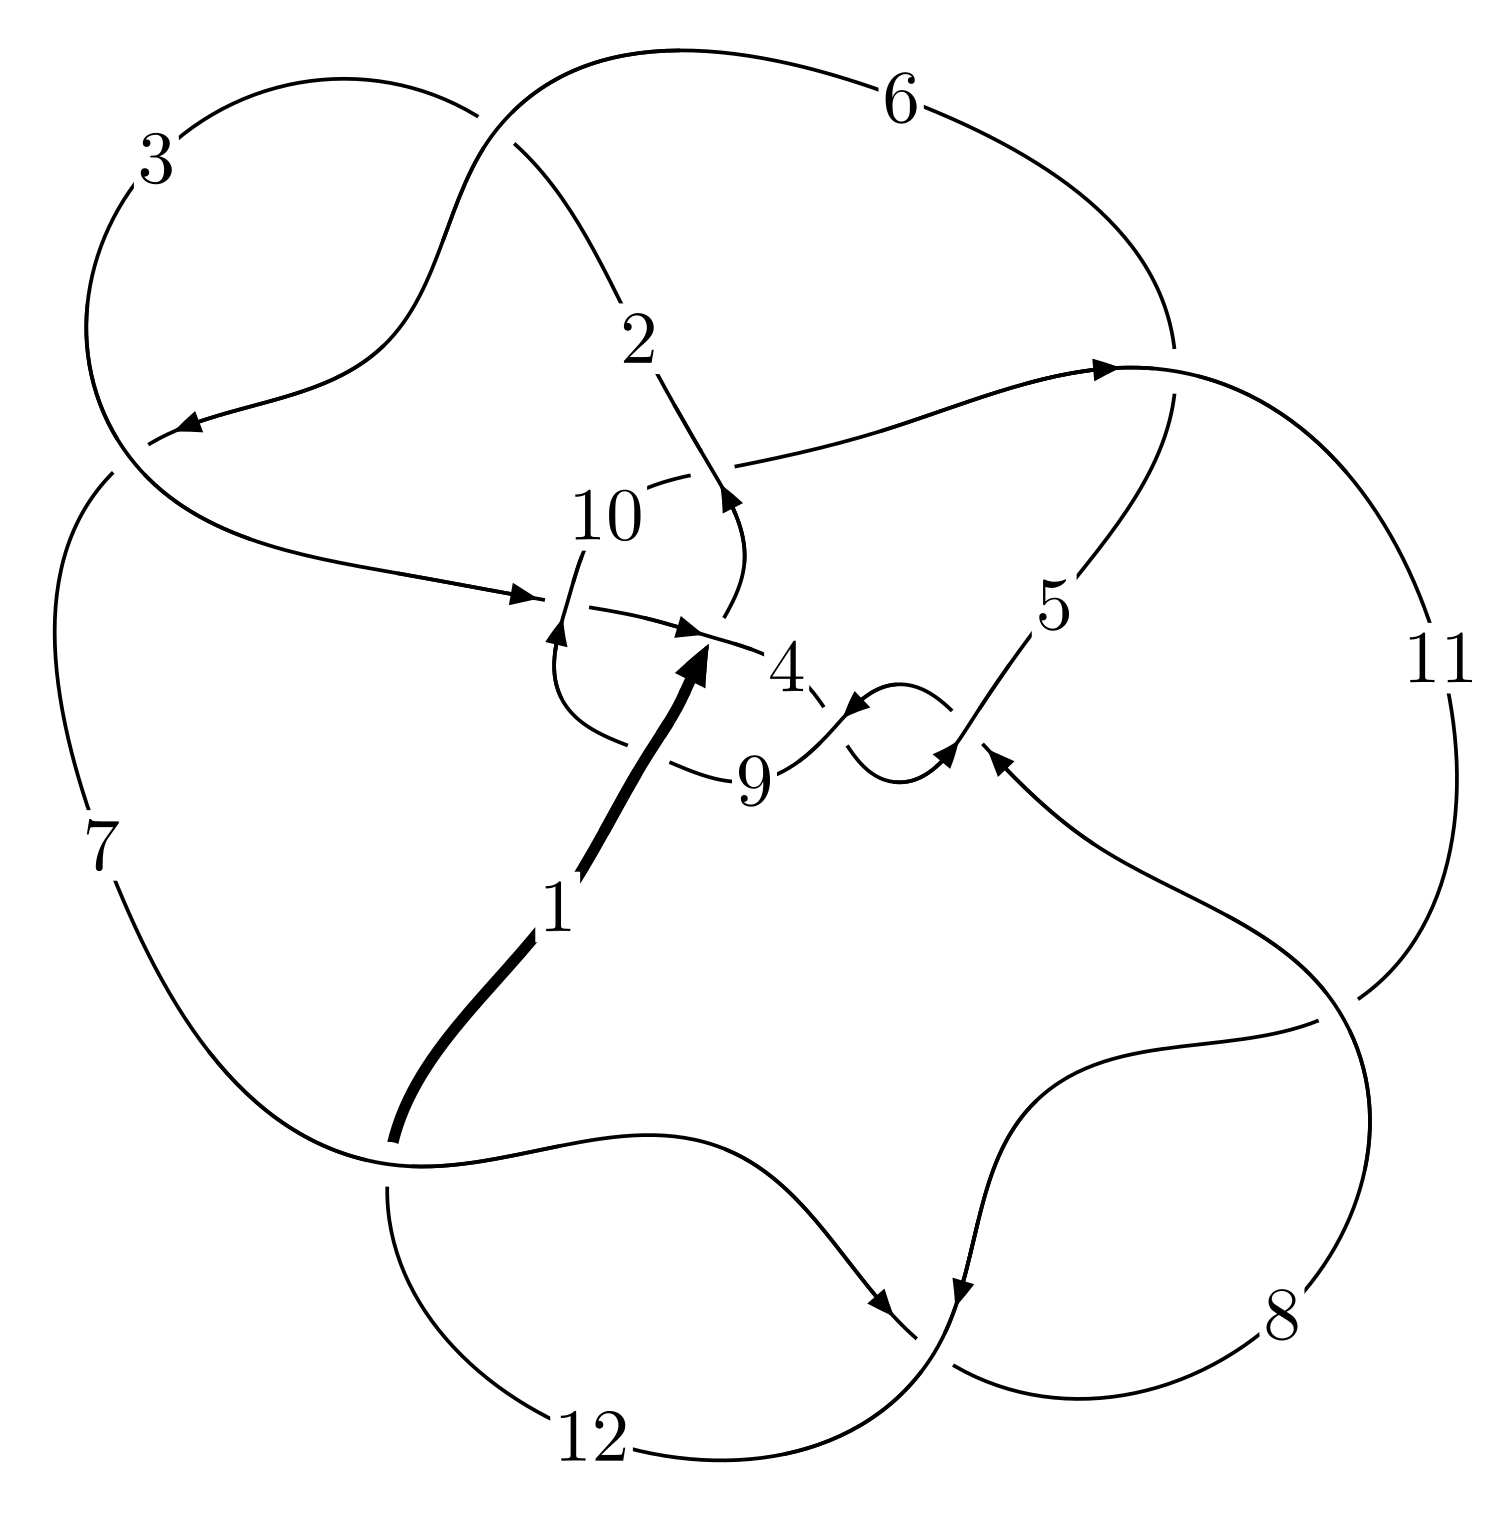
\includegraphics[width=112pt]{../../../GIT/diagram.site/Diagrams/png/1756_12a_0955.png}\\
\ \ \ A knot diagram\footnotemark}&
\allowdisplaybreaks
\textbf{Linearized knot diagam} \\
\cline{2-2}
 &
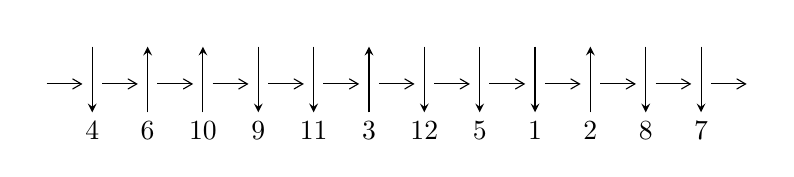
\begin{tikzpicture}[x=20pt, y=17pt]
	% nodes
	\node (C0) at (0, 0) {};
	\node (C1) at (1, 0) {};
	\node (C1U) at (1, +1) {};
	\node (C1D) at (1, -1) {4};

	\node (C2) at (2, 0) {};
	\node (C2U) at (2, +1) {};
	\node (C2D) at (2, -1) {6};

	\node (C3) at (3, 0) {};
	\node (C3U) at (3, +1) {};
	\node (C3D) at (3, -1) {10};

	\node (C4) at (4, 0) {};
	\node (C4U) at (4, +1) {};
	\node (C4D) at (4, -1) {9};

	\node (C5) at (5, 0) {};
	\node (C5U) at (5, +1) {};
	\node (C5D) at (5, -1) {11};

	\node (C6) at (6, 0) {};
	\node (C6U) at (6, +1) {};
	\node (C6D) at (6, -1) {3};

	\node (C7) at (7, 0) {};
	\node (C7U) at (7, +1) {};
	\node (C7D) at (7, -1) {12};

	\node (C8) at (8, 0) {};
	\node (C8U) at (8, +1) {};
	\node (C8D) at (8, -1) {5};

	\node (C9) at (9, 0) {};
	\node (C9U) at (9, +1) {};
	\node (C9D) at (9, -1) {1};

	\node (C10) at (10, 0) {};
	\node (C10U) at (10, +1) {};
	\node (C10D) at (10, -1) {2};

	\node (C11) at (11, 0) {};
	\node (C11U) at (11, +1) {};
	\node (C11D) at (11, -1) {8};

	\node (C12) at (12, 0) {};
	\node (C12U) at (12, +1) {};
	\node (C12D) at (12, -1) {7};
	\node (C13) at (13, 0) {};

	% arrows
	\draw[->,>={angle 60}]
	(C0) edge (C1) (C1) edge (C2) (C2) edge (C3) (C3) edge (C4) (C4) edge (C5) (C5) edge (C6) (C6) edge (C7) (C7) edge (C8) (C8) edge (C9) (C9) edge (C10) (C10) edge (C11) (C11) edge (C12) (C12) edge (C13) ;	\draw[->,>=stealth]
	(C1U) edge (C1D) (C2D) edge (C2U) (C3D) edge (C3U) (C4U) edge (C4D) (C5U) edge (C5D) (C6D) edge (C6U) (C7U) edge (C7D) (C8U) edge (C8D) (C9U) edge (C9D) (C10D) edge (C10U) (C11U) edge (C11D) (C12U) edge (C12D) ;
	\end{tikzpicture} \\
\hhline{~~} \\& 
\textbf{Solving Sequence} \\ \cline{2-2} 
 &
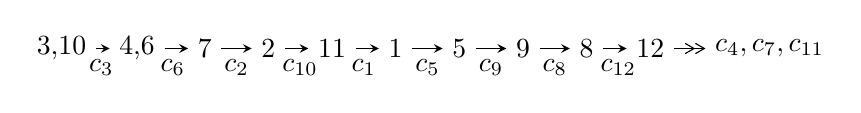
\begin{tikzpicture}[x=23pt, y=7pt]
	% node
	\node (A0) at (-1/8, 0) {3,10};
	\node (A1) at (17/16, 0) {4,6};
	\node (A2) at (17/8, 0) {7};
	\node (A3) at (25/8, 0) {2};
	\node (A4) at (33/8, 0) {11};
	\node (A5) at (41/8, 0) {1};
	\node (A6) at (49/8, 0) {5};
	\node (A7) at (57/8, 0) {9};
	\node (A8) at (65/8, 0) {8};
	\node (A9) at (73/8, 0) {12};
	\node (C1) at (1/2, -1) {$c_{3}$};
	\node (C2) at (13/8, -1) {$c_{6}$};
	\node (C3) at (21/8, -1) {$c_{2}$};
	\node (C4) at (29/8, -1) {$c_{10}$};
	\node (C5) at (37/8, -1) {$c_{1}$};
	\node (C6) at (45/8, -1) {$c_{5}$};
	\node (C7) at (53/8, -1) {$c_{9}$};
	\node (C8) at (61/8, -1) {$c_{8}$};
	\node (C9) at (69/8, -1) {$c_{12}$};
	\node (A10) at (11, 0) {$c_{4},c_{7},c_{11}$};

	% edge
	\draw[->,>=stealth]	
	(A0) edge (A1) (A1) edge (A2) (A2) edge (A3) (A3) edge (A4) (A4) edge (A5) (A5) edge (A6) (A6) edge (A7) (A7) edge (A8) (A8) edge (A9) ;
	\draw[->>,>={angle 60}]	
	(A9) edge (A10);
\end{tikzpicture} \\ 

\end{tabular} \\

\footnotetext{
The image of knot diagram is generated by the software ``\textbf{Draw programme}" developed by Andrew Bartholomew(\url{http://www.layer8.co.uk/maths/draw/index.htm\#Running-draw}), where we modified some parts for our purpose(\url{https://github.com/CATsTAILs/LinksPainter}).
}\phantom \\ \newline 
\centering \textbf{Ideals for irreducible components\footnotemark of $X_{\text{par}}$} 
 
\begin{align*}
I^u_{1}&=\langle 
-9.91588\times10^{1054} u^{135}+6.69620\times10^{1054} u^{134}+\cdots+1.75763\times10^{1054} b+3.05109\times10^{1055},\\
\phantom{I^u_{1}}&\phantom{= \langle  }-2.92192\times10^{1056} u^{135}+2.42676\times10^{1056} u^{134}+\cdots+1.75763\times10^{1054} a+1.61676\times10^{1057},\\
\phantom{I^u_{1}}&\phantom{= \langle  }u^{136}- u^{135}+\cdots-90 u+1\rangle \\
I^u_{2}&=\langle 
1.29910\times10^{75} u^{39}+6.04417\times10^{73} u^{38}+\cdots+7.64937\times10^{75} b-2.92334\times10^{75},\\
\phantom{I^u_{2}}&\phantom{= \langle  }3.00344\times10^{74} u^{39}+4.01392\times10^{74} u^{38}+\cdots+7.64937\times10^{75} a+1.89389\times10^{76},\;u^{40}+6 u^{38}+\cdots+2 u+1\rangle \\
\\
\end{align*}
\raggedright * 2 irreducible components of $\dim_{\mathbb{C}}=0$, with total 176 representations.\\
\footnotetext{All coefficients of polynomials are rational numbers. But the coefficients are sometimes approximated in decimal forms when there is not enough margin.}
\newpage
\renewcommand{\arraystretch}{1}
\centering \section*{I. $I^u_{1}= \langle -9.92\times10^{1054} u^{135}+6.70\times10^{1054} u^{134}+\cdots+1.76\times10^{1054} b+3.05\times10^{1055},\;-2.92\times10^{1056} u^{135}+2.43\times10^{1056} u^{134}+\cdots+1.76\times10^{1054} a+1.62\times10^{1057},\;u^{136}- u^{135}+\cdots-90 u+1 \rangle$}
\flushleft \textbf{(i) Arc colorings}\\
\begin{tabular}{m{7pt} m{180pt} m{7pt} m{180pt} }
\flushright $a_{3}=$&$\begin{pmatrix}1\\0\end{pmatrix}$ \\
\flushright $a_{10}=$&$\begin{pmatrix}0\\u\end{pmatrix}$ \\
\flushright $a_{4}=$&$\begin{pmatrix}1\\- u^2\end{pmatrix}$ \\
\flushright $a_{6}=$&$\begin{pmatrix}166.241 u^{135}-138.070 u^{134}+\cdots+84755.9 u-919.851\\5.64160 u^{135}-3.80978 u^{134}+\cdots+1561.92 u-17.3591\end{pmatrix}$ \\
\flushright $a_{7}=$&$\begin{pmatrix}171.883 u^{135}-141.880 u^{134}+\cdots+86317.8 u-937.210\\5.64160 u^{135}-3.80978 u^{134}+\cdots+1561.92 u-17.3591\end{pmatrix}$ \\
\flushright $a_{2}=$&$\begin{pmatrix}-112.241 u^{135}+97.0441 u^{134}+\cdots-67403.4 u+879.171\\10.4249 u^{135}-6.60479 u^{134}+\cdots+1875.62 u-20.2786\end{pmatrix}$ \\
\flushright $a_{11}=$&$\begin{pmatrix}-160.594 u^{135}+137.593 u^{134}+\cdots-96574.1 u+1237.25\\-0.205345 u^{135}+2.30610 u^{134}+\cdots-3591.94 u+45.2540\end{pmatrix}$ \\
\flushright $a_{1}=$&$\begin{pmatrix}-103.598 u^{135}+92.1701 u^{134}+\cdots-66783.3 u+874.089\\9.12403 u^{135}-5.70219 u^{134}+\cdots+1545.05 u-16.5096\end{pmatrix}$ \\
\flushright $a_{5}=$&$\begin{pmatrix}147.567 u^{135}-121.755 u^{134}+\cdots+73520.8 u-834.757\\0.975785 u^{135}+0.194203 u^{134}+\cdots-1776.12 u+23.0939\end{pmatrix}$ \\
\flushright $a_{9}=$&$\begin{pmatrix}-175.798 u^{135}+152.843 u^{134}+\cdots-109261. u+1393.02\\-8.58222 u^{135}+7.48626 u^{134}+\cdots-5293.45 u+64.5618\end{pmatrix}$ \\
\flushright $a_{8}=$&$\begin{pmatrix}163.248 u^{135}-136.229 u^{134}+\cdots+85190.3 u-925.173\\6.21223 u^{135}-4.81821 u^{134}+\cdots+2835.38 u-33.0506\end{pmatrix}$ \\
\flushright $a_{12}=$&$\begin{pmatrix}35.9075 u^{135}-30.6827 u^{134}+\cdots+21883.0 u-266.266\\-0.370479 u^{135}-0.414086 u^{134}+\cdots+989.079 u-12.4810\end{pmatrix}$\\&\end{tabular}
\flushleft \textbf{(ii) Obstruction class $= -1$}\\~\\
\flushleft \textbf{(iii) Cusp Shapes $= -178.426 u^{135}+121.516 u^{134}+\cdots-41107.4 u+451.503$}\\~\\
\newpage\renewcommand{\arraystretch}{1}
\flushleft \textbf{(iv) u-Polynomials at the component}\newline \\
\begin{tabular}{m{50pt}|m{274pt}}
Crossings & \hspace{64pt}u-Polynomials at each crossing \\
\hline $$\begin{aligned}c_{1}\end{aligned}$$&$\begin{aligned}
&u^{136}-11 u^{135}+\cdots-99138 u+6727
\end{aligned}$\\
\hline $$\begin{aligned}c_{2},c_{6}\end{aligned}$$&$\begin{aligned}
&u^{136}-3 u^{135}+\cdots-1044 u+4261
\end{aligned}$\\
\hline $$\begin{aligned}c_{3}\end{aligned}$$&$\begin{aligned}
&u^{136}+u^{135}+\cdots+90 u+1
\end{aligned}$\\
\hline $$\begin{aligned}c_{4},c_{8}\end{aligned}$$&$\begin{aligned}
&u^{136}+4 u^{135}+\cdots-238658 u+29957
\end{aligned}$\\
\hline $$\begin{aligned}c_{5}\end{aligned}$$&$\begin{aligned}
&u^{136}+u^{135}+\cdots-958173436 u+138684577
\end{aligned}$\\
\hline $$\begin{aligned}c_{7},c_{11},c_{12}\end{aligned}$$&$\begin{aligned}
&u^{136}+72 u^{134}+\cdots-558 u+71
\end{aligned}$\\
\hline $$\begin{aligned}c_{9}\end{aligned}$$&$\begin{aligned}
&u^{136}+19 u^{134}+\cdots-157163 u+21971
\end{aligned}$\\
\hline $$\begin{aligned}c_{10}\end{aligned}$$&$\begin{aligned}
&u^{136}-15 u^{134}+\cdots+28235809 u+4063723
\end{aligned}$\\
\hline
\end{tabular}\\~\\
\newpage\renewcommand{\arraystretch}{1}
\flushleft \textbf{(v) Riley Polynomials at the component}\newline \\
\begin{tabular}{m{50pt}|m{274pt}}
Crossings & \hspace{64pt}Riley Polynomials at each crossing \\
\hline $$\begin{aligned}c_{1}\end{aligned}$$&$\begin{aligned}
&y^{136}+33 y^{135}+\cdots+1941216156 y+45252529
\end{aligned}$\\
\hline $$\begin{aligned}c_{2},c_{6}\end{aligned}$$&$\begin{aligned}
&y^{136}-89 y^{135}+\cdots-722664720 y+18156121
\end{aligned}$\\
\hline $$\begin{aligned}c_{3}\end{aligned}$$&$\begin{aligned}
&y^{136}+5 y^{135}+\cdots-3718 y+1
\end{aligned}$\\
\hline $$\begin{aligned}c_{4},c_{8}\end{aligned}$$&$\begin{aligned}
&y^{136}+122 y^{135}+\cdots-20806491988 y+897421849
\end{aligned}$\\
\hline $$\begin{aligned}c_{5}\end{aligned}$$&$\begin{aligned}
&y^{136}+79 y^{135}+\cdots+1981830159489008108 y+19233411897668929
\end{aligned}$\\
\hline $$\begin{aligned}c_{7},c_{11},c_{12}\end{aligned}$$&$\begin{aligned}
&y^{136}+144 y^{135}+\cdots+122872 y+5041
\end{aligned}$\\
\hline $$\begin{aligned}c_{9}\end{aligned}$$&$\begin{aligned}
&y^{136}+38 y^{135}+\cdots+7897021639 y+482724841
\end{aligned}$\\
\hline $$\begin{aligned}c_{10}\end{aligned}$$&$\begin{aligned}
&y^{136}-30 y^{135}+\cdots-461058800492953 y+16513844620729
\end{aligned}$\\
\hline
\end{tabular}\\~\\
\newpage\flushleft \textbf{(vi) Complex Volumes and Cusp Shapes}
$$\begin{array}{c|c|c}  
\text{Solutions to }I^u_{1}& \I (\text{vol} + \sqrt{-1}CS) & \text{Cusp shape}\\
 \hline 
\begin{aligned}
u &= -1.002500 + 0.063014 I \\
a &= \phantom{-}2.26750 - 0.41171 I \\
b &= -1.233320 + 0.422915 I\end{aligned}
 & \phantom{-}14.1826 - 7.7014 I & \phantom{-0.000000 } 0 \\ \hline\begin{aligned}
u &= -1.002500 - 0.063014 I \\
a &= \phantom{-}2.26750 + 0.41171 I \\
b &= -1.233320 - 0.422915 I\end{aligned}
 & \phantom{-}14.1826 + 7.7014 I & \phantom{-0.000000 } 0 \\ \hline\begin{aligned}
u &= -0.268691 + 0.984175 I \\
a &= \phantom{-}0.504189 + 0.133192 I \\
b &= \phantom{-}0.318734 + 0.297660 I\end{aligned}
 & -0.41282 - 1.61897 I & \phantom{-0.000000 } 0 \\ \hline\begin{aligned}
u &= -0.268691 - 0.984175 I \\
a &= \phantom{-}0.504189 - 0.133192 I \\
b &= \phantom{-}0.318734 - 0.297660 I\end{aligned}
 & -0.41282 + 1.61897 I & \phantom{-0.000000 } 0 \\ \hline\begin{aligned}
u &= \phantom{-}0.605736 + 0.838936 I \\
a &= -0.728686 + 0.627850 I \\
b &= -0.409253 + 0.667357 I\end{aligned}
 & \phantom{-}3.53391 - 2.67721 I & \phantom{-0.000000 } 0 \\ \hline\begin{aligned}
u &= \phantom{-}0.605736 - 0.838936 I \\
a &= -0.728686 - 0.627850 I \\
b &= -0.409253 - 0.667357 I\end{aligned}
 & \phantom{-}3.53391 + 2.67721 I & \phantom{-0.000000 } 0 \\ \hline\begin{aligned}
u &= -0.479470 + 0.830260 I \\
a &= -0.438130 - 0.008324 I \\
b &= \phantom{-}0.432698 - 0.924634 I\end{aligned}
 & \phantom{-}2.55578 - 3.30889 I & \phantom{-0.000000 } 0 \\ \hline\begin{aligned}
u &= -0.479470 - 0.830260 I \\
a &= -0.438130 + 0.008324 I \\
b &= \phantom{-}0.432698 + 0.924634 I\end{aligned}
 & \phantom{-}2.55578 + 3.30889 I & \phantom{-0.000000 } 0 \\ \hline\begin{aligned}
u &= \phantom{-}0.816298 + 0.498199 I \\
a &= \phantom{-}2.30208 - 1.08177 I \\
b &= -1.095330 - 0.444551 I\end{aligned}
 & \phantom{-}6.58510 + 5.02708 I & \phantom{-0.000000 } 0 \\ \hline\begin{aligned}
u &= \phantom{-}0.816298 - 0.498199 I \\
a &= \phantom{-}2.30208 + 1.08177 I \\
b &= -1.095330 + 0.444551 I\end{aligned}
 & \phantom{-}6.58510 - 5.02708 I & \phantom{-0.000000 } 0\\
 \hline 
 \end{array}$$\newpage$$\begin{array}{c|c|c}  
\text{Solutions to }I^u_{1}& \I (\text{vol} + \sqrt{-1}CS) & \text{Cusp shape}\\
 \hline 
\begin{aligned}
u &= -0.727375 + 0.755504 I \\
a &= \phantom{-}0.351811 - 0.182094 I \\
b &= -0.616455 - 1.037090 I\end{aligned}
 & \phantom{-}6.10494 + 2.29566 I & \phantom{-0.000000 } 0 \\ \hline\begin{aligned}
u &= -0.727375 - 0.755504 I \\
a &= \phantom{-}0.351811 + 0.182094 I \\
b &= -0.616455 + 1.037090 I\end{aligned}
 & \phantom{-}6.10494 - 2.29566 I & \phantom{-0.000000 } 0 \\ \hline\begin{aligned}
u &= -0.389122 + 0.843441 I \\
a &= \phantom{-}0.321785 - 0.000734 I \\
b &= \phantom{-}0.062580 + 0.521542 I\end{aligned}
 & -0.36394 - 1.54443 I & \phantom{-0.000000 } 0 \\ \hline\begin{aligned}
u &= -0.389122 - 0.843441 I \\
a &= \phantom{-}0.321785 + 0.000734 I \\
b &= \phantom{-}0.062580 - 0.521542 I\end{aligned}
 & -0.36394 + 1.54443 I & \phantom{-0.000000 } 0 \\ \hline\begin{aligned}
u &= -0.398424 + 0.801121 I \\
a &= -0.621530 + 0.078693 I \\
b &= -0.418336 + 0.507954 I\end{aligned}
 & \phantom{-}0.74586 - 4.82761 I & \phantom{-0.000000 } 0 \\ \hline\begin{aligned}
u &= -0.398424 - 0.801121 I \\
a &= -0.621530 - 0.078693 I \\
b &= -0.418336 - 0.507954 I\end{aligned}
 & \phantom{-}0.74586 + 4.82761 I & \phantom{-0.000000 } 0 \\ \hline\begin{aligned}
u &= -0.658120 + 0.599733 I \\
a &= -1.39914 - 0.59882 I \\
b &= \phantom{-}1.47290 - 0.66787 I\end{aligned}
 & \phantom{-}12.7343 - 10.3334 I & \phantom{-0.000000 } 0 \\ \hline\begin{aligned}
u &= -0.658120 - 0.599733 I \\
a &= -1.39914 + 0.59882 I \\
b &= \phantom{-}1.47290 + 0.66787 I\end{aligned}
 & \phantom{-}12.7343 + 10.3334 I & \phantom{-0.000000 } 0 \\ \hline\begin{aligned}
u &= -1.048210 + 0.371939 I \\
a &= -1.86845 - 0.10856 I \\
b &= \phantom{-}1.324620 - 0.352471 I\end{aligned}
 & \phantom{-}10.73120 - 5.00750 I & \phantom{-0.000000 } 0 \\ \hline\begin{aligned}
u &= -1.048210 - 0.371939 I \\
a &= -1.86845 + 0.10856 I \\
b &= \phantom{-}1.324620 + 0.352471 I\end{aligned}
 & \phantom{-}10.73120 + 5.00750 I & \phantom{-0.000000 } 0\\
 \hline 
 \end{array}$$\newpage$$\begin{array}{c|c|c}  
\text{Solutions to }I^u_{1}& \I (\text{vol} + \sqrt{-1}CS) & \text{Cusp shape}\\
 \hline 
\begin{aligned}
u &= -0.712861 + 0.488127 I \\
a &= -0.412892 + 0.500570 I \\
b &= -0.167658 - 0.583468 I\end{aligned}
 & \phantom{-}4.00300 - 1.05980 I & \phantom{-0.000000 } 0 \\ \hline\begin{aligned}
u &= -0.712861 - 0.488127 I \\
a &= -0.412892 - 0.500570 I \\
b &= -0.167658 + 0.583468 I\end{aligned}
 & \phantom{-}4.00300 + 1.05980 I & \phantom{-0.000000 } 0 \\ \hline\begin{aligned}
u &= -0.187510 + 0.833352 I \\
a &= \phantom{-}0.840276 - 0.688063 I \\
b &= \phantom{-}0.813280 - 0.195468 I\end{aligned}
 & -0.70171 - 2.24730 I & \phantom{-0.000000 } 0 \\ \hline\begin{aligned}
u &= -0.187510 - 0.833352 I \\
a &= \phantom{-}0.840276 + 0.688063 I \\
b &= \phantom{-}0.813280 + 0.195468 I\end{aligned}
 & -0.70171 + 2.24730 I & \phantom{-0.000000 } 0 \\ \hline\begin{aligned}
u &= \phantom{-}0.239091 + 0.819586 I \\
a &= -1.47388 - 0.99592 I \\
b &= -1.151490 - 0.233690 I\end{aligned}
 & \phantom{-}11.5671 + 8.5371 I & \phantom{-0.000000 } 0 \\ \hline\begin{aligned}
u &= \phantom{-}0.239091 - 0.819586 I \\
a &= -1.47388 + 0.99592 I \\
b &= -1.151490 + 0.233690 I\end{aligned}
 & \phantom{-}11.5671 - 8.5371 I & \phantom{-0.000000 } 0 \\ \hline\begin{aligned}
u &= -0.793679 + 0.163901 I \\
a &= \phantom{-}0.403955 + 1.273500 I \\
b &= \phantom{-}0.259003 + 0.463813 I\end{aligned}
 & \phantom{-}3.19544 - 2.72879 I & \phantom{-0.000000 } 0 \\ \hline\begin{aligned}
u &= -0.793679 - 0.163901 I \\
a &= \phantom{-}0.403955 - 1.273500 I \\
b &= \phantom{-}0.259003 - 0.463813 I\end{aligned}
 & \phantom{-}3.19544 + 2.72879 I & \phantom{-0.000000 } 0 \\ \hline\begin{aligned}
u &= -0.088010 + 0.799434 I \\
a &= -2.24733 + 0.36788 I \\
b &= -1.039660 + 0.072164 I\end{aligned}
 & \phantom{-}3.55213 - 3.56061 I & \phantom{-0.000000 } 0 \\ \hline\begin{aligned}
u &= -0.088010 - 0.799434 I \\
a &= -2.24733 - 0.36788 I \\
b &= -1.039660 - 0.072164 I\end{aligned}
 & \phantom{-}3.55213 + 3.56061 I & \phantom{-0.000000 } 0\\
 \hline 
 \end{array}$$\newpage$$\begin{array}{c|c|c}  
\text{Solutions to }I^u_{1}& \I (\text{vol} + \sqrt{-1}CS) & \text{Cusp shape}\\
 \hline 
\begin{aligned}
u &= \phantom{-}0.887942 + 0.814621 I \\
a &= \phantom{-}0.066964 - 0.228052 I \\
b &= \phantom{-}0.129749 - 1.058500 I\end{aligned}
 & -1.56586 + 3.74407 I & \phantom{-0.000000 } 0 \\ \hline\begin{aligned}
u &= \phantom{-}0.887942 - 0.814621 I \\
a &= \phantom{-}0.066964 + 0.228052 I \\
b &= \phantom{-}0.129749 + 1.058500 I\end{aligned}
 & -1.56586 - 3.74407 I & \phantom{-0.000000 } 0 \\ \hline\begin{aligned}
u &= -0.692156 + 0.990198 I \\
a &= \phantom{-}1.47593 + 0.13370 I \\
b &= -0.878064 - 0.164448 I\end{aligned}
 & \phantom{-}4.10114 + 0.66022 I & \phantom{-0.000000 } 0 \\ \hline\begin{aligned}
u &= -0.692156 - 0.990198 I \\
a &= \phantom{-}1.47593 - 0.13370 I \\
b &= -0.878064 + 0.164448 I\end{aligned}
 & \phantom{-}4.10114 - 0.66022 I & \phantom{-0.000000 } 0 \\ \hline\begin{aligned}
u &= -1.027430 + 0.637510 I \\
a &= \phantom{-}1.60176 + 0.29050 I \\
b &= -1.50451 + 0.23809 I\end{aligned}
 & \phantom{-}16.3588 - 3.0418 I & \phantom{-0.000000 } 0 \\ \hline\begin{aligned}
u &= -1.027430 - 0.637510 I \\
a &= \phantom{-}1.60176 - 0.29050 I \\
b &= -1.50451 - 0.23809 I\end{aligned}
 & \phantom{-}16.3588 + 3.0418 I & \phantom{-0.000000 } 0 \\ \hline\begin{aligned}
u &= -0.553504 + 0.558455 I \\
a &= \phantom{-}1.008670 + 0.672872 I \\
b &= -0.980509 + 0.372582 I\end{aligned}
 & \phantom{-}1.89932 - 1.74077 I & \phantom{-0.000000 } 0 \\ \hline\begin{aligned}
u &= -0.553504 - 0.558455 I \\
a &= \phantom{-}1.008670 - 0.672872 I \\
b &= -0.980509 - 0.372582 I\end{aligned}
 & \phantom{-}1.89932 + 1.74077 I & \phantom{-0.000000 } 0 \\ \hline\begin{aligned}
u &= \phantom{-}0.121197 + 0.762928 I \\
a &= \phantom{-}0.541844 + 0.084245 I \\
b &= -0.014393 + 0.583516 I\end{aligned}
 & -0.80117 - 1.41412 I & \phantom{-0.000000 } 0 \\ \hline\begin{aligned}
u &= \phantom{-}0.121197 - 0.762928 I \\
a &= \phantom{-}0.541844 - 0.084245 I \\
b &= -0.014393 - 0.583516 I\end{aligned}
 & -0.80117 + 1.41412 I & \phantom{-0.000000 } 0\\
 \hline 
 \end{array}$$\newpage$$\begin{array}{c|c|c}  
\text{Solutions to }I^u_{1}& \I (\text{vol} + \sqrt{-1}CS) & \text{Cusp shape}\\
 \hline 
\begin{aligned}
u &= -0.596209 + 0.479918 I \\
a &= \phantom{-}1.39245 + 1.03343 I \\
b &= -1.34852 + 0.65533 I\end{aligned}
 & \phantom{-}8.40609 - 5.75438 I & \phantom{-0.000000 } 0 \\ \hline\begin{aligned}
u &= -0.596209 - 0.479918 I \\
a &= \phantom{-}1.39245 - 1.03343 I \\
b &= -1.34852 - 0.65533 I\end{aligned}
 & \phantom{-}8.40609 + 5.75438 I & \phantom{-0.000000 } 0 \\ \hline\begin{aligned}
u &= -0.660020 + 0.385811 I \\
a &= -1.178570 - 0.050631 I \\
b &= \phantom{-}1.39664 + 0.63986 I\end{aligned}
 & \phantom{-}7.54221 - 2.75018 I & \phantom{-0.000000 } 0 \\ \hline\begin{aligned}
u &= -0.660020 - 0.385811 I \\
a &= -1.178570 + 0.050631 I \\
b &= \phantom{-}1.39664 - 0.63986 I\end{aligned}
 & \phantom{-}7.54221 + 2.75018 I & \phantom{-0.000000 } 0 \\ \hline\begin{aligned}
u &= \phantom{-}0.837017 + 0.915713 I \\
a &= -0.226742 + 0.092602 I \\
b &= -0.014695 + 1.060940 I\end{aligned}
 & \phantom{-}3.44137 + 8.50029 I & \phantom{-0.000000 } 0 \\ \hline\begin{aligned}
u &= \phantom{-}0.837017 - 0.915713 I \\
a &= -0.226742 - 0.092602 I \\
b &= -0.014695 - 1.060940 I\end{aligned}
 & \phantom{-}3.44137 - 8.50029 I & \phantom{-0.000000 } 0 \\ \hline\begin{aligned}
u &= \phantom{-}0.565967 + 1.144860 I \\
a &= -0.094721 + 0.616456 I \\
b &= \phantom{-}1.008800 + 0.175200 I\end{aligned}
 & \phantom{-}5.15870 + 5.32280 I & \phantom{-0.000000 } 0 \\ \hline\begin{aligned}
u &= \phantom{-}0.565967 - 1.144860 I \\
a &= -0.094721 - 0.616456 I \\
b &= \phantom{-}1.008800 - 0.175200 I\end{aligned}
 & \phantom{-}5.15870 - 5.32280 I & \phantom{-0.000000 } 0 \\ \hline\begin{aligned}
u &= \phantom{-}0.958967 + 0.871863 I \\
a &= -1.55424 + 0.69528 I \\
b &= \phantom{-}1.187340 + 0.441105 I\end{aligned}
 & \phantom{-}2.79943 + 5.61282 I & \phantom{-0.000000 } 0 \\ \hline\begin{aligned}
u &= \phantom{-}0.958967 - 0.871863 I \\
a &= -1.55424 - 0.69528 I \\
b &= \phantom{-}1.187340 - 0.441105 I\end{aligned}
 & \phantom{-}2.79943 - 5.61282 I & \phantom{-0.000000 } 0\\
 \hline 
 \end{array}$$\newpage$$\begin{array}{c|c|c}  
\text{Solutions to }I^u_{1}& \I (\text{vol} + \sqrt{-1}CS) & \text{Cusp shape}\\
 \hline 
\begin{aligned}
u &= -0.765743 + 1.085720 I \\
a &= -0.328234 - 0.289606 I \\
b &= \phantom{-}0.562214 + 0.242411 I\end{aligned}
 & \phantom{-}1.30346 - 3.92039 I & \phantom{-0.000000 } 0 \\ \hline\begin{aligned}
u &= -0.765743 - 1.085720 I \\
a &= -0.328234 + 0.289606 I \\
b &= \phantom{-}0.562214 - 0.242411 I\end{aligned}
 & \phantom{-}1.30346 + 3.92039 I & \phantom{-0.000000 } 0 \\ \hline\begin{aligned}
u &= \phantom{-}0.791285 + 1.067280 I \\
a &= -1.143380 + 0.775089 I \\
b &= \phantom{-}1.150870 - 0.080158 I\end{aligned}
 & \phantom{-}7.61172 - 0.99607 I & \phantom{-0.000000 } 0 \\ \hline\begin{aligned}
u &= \phantom{-}0.791285 - 1.067280 I \\
a &= -1.143380 - 0.775089 I \\
b &= \phantom{-}1.150870 + 0.080158 I\end{aligned}
 & \phantom{-}7.61172 + 0.99607 I & \phantom{-0.000000 } 0 \\ \hline\begin{aligned}
u &= \phantom{-}0.785394 + 1.073990 I \\
a &= -0.427491 + 0.713269 I \\
b &= \phantom{-}0.910080 + 0.222265 I\end{aligned}
 & \phantom{-}5.10789 + 5.30901 I & \phantom{-0.000000 } 0 \\ \hline\begin{aligned}
u &= \phantom{-}0.785394 - 1.073990 I \\
a &= -0.427491 - 0.713269 I \\
b &= \phantom{-}0.910080 - 0.222265 I\end{aligned}
 & \phantom{-}5.10789 - 5.30901 I & \phantom{-0.000000 } 0 \\ \hline\begin{aligned}
u &= \phantom{-}0.615778 + 0.258179 I \\
a &= \phantom{-}0.48844 - 1.51099 I \\
b &= \phantom{-}0.100617 + 0.656427 I\end{aligned}
 & \phantom{-}10.40450 + 3.59236 I & \phantom{-0.000000 } 0 \\ \hline\begin{aligned}
u &= \phantom{-}0.615778 - 0.258179 I \\
a &= \phantom{-}0.48844 + 1.51099 I \\
b &= \phantom{-}0.100617 - 0.656427 I\end{aligned}
 & \phantom{-}10.40450 - 3.59236 I & \phantom{-0.000000 } 0 \\ \hline\begin{aligned}
u &= \phantom{-}1.299960 + 0.324998 I \\
a &= -1.083360 - 0.026428 I \\
b &= \phantom{-}1.63019 - 0.35452 I\end{aligned}
 & \phantom{-}16.8741 + 5.7954 I & \phantom{-0.000000 } 0 \\ \hline\begin{aligned}
u &= \phantom{-}1.299960 - 0.324998 I \\
a &= -1.083360 + 0.026428 I \\
b &= \phantom{-}1.63019 + 0.35452 I\end{aligned}
 & \phantom{-}16.8741 - 5.7954 I & \phantom{-0.000000 } 0\\
 \hline 
 \end{array}$$\newpage$$\begin{array}{c|c|c}  
\text{Solutions to }I^u_{1}& \I (\text{vol} + \sqrt{-1}CS) & \text{Cusp shape}\\
 \hline 
\begin{aligned}
u &= -1.250060 + 0.491063 I \\
a &= \phantom{-}1.195670 + 0.003182 I \\
b &= -1.228970 - 0.245647 I\end{aligned}
 & \phantom{-}3.66584 + 0.57684 I & \phantom{-0.000000 } 0 \\ \hline\begin{aligned}
u &= -1.250060 - 0.491063 I \\
a &= \phantom{-}1.195670 - 0.003182 I \\
b &= -1.228970 + 0.245647 I\end{aligned}
 & \phantom{-}3.66584 - 0.57684 I & \phantom{-0.000000 } 0 \\ \hline\begin{aligned}
u &= \phantom{-}0.946176 + 0.971207 I \\
a &= \phantom{-}0.961632 - 0.604019 I \\
b &= -0.953124 - 0.659253 I\end{aligned}
 & \phantom{-}7.32100 + 3.63789 I & \phantom{-0.000000 } 0 \\ \hline\begin{aligned}
u &= \phantom{-}0.946176 - 0.971207 I \\
a &= \phantom{-}0.961632 + 0.604019 I \\
b &= -0.953124 + 0.659253 I\end{aligned}
 & \phantom{-}7.32100 - 3.63789 I & \phantom{-0.000000 } 0 \\ \hline\begin{aligned}
u &= \phantom{-}0.970389 + 0.962515 I \\
a &= \phantom{-}1.48843 - 0.67039 I \\
b &= -1.37225 - 0.39614 I\end{aligned}
 & \phantom{-}7.91599 + 7.79466 I & \phantom{-0.000000 } 0 \\ \hline\begin{aligned}
u &= \phantom{-}0.970389 - 0.962515 I \\
a &= \phantom{-}1.48843 + 0.67039 I \\
b &= -1.37225 + 0.39614 I\end{aligned}
 & \phantom{-}7.91599 - 7.79466 I & \phantom{-0.000000 } 0 \\ \hline\begin{aligned}
u &= -0.326293 + 1.331470 I \\
a &= \phantom{-}0.391756 - 0.149787 I \\
b &= -0.733453 - 0.039222 I\end{aligned}
 & -0.181456 - 0.824990 I & \phantom{-0.000000 } 0 \\ \hline\begin{aligned}
u &= -0.326293 - 1.331470 I \\
a &= \phantom{-}0.391756 + 0.149787 I \\
b &= -0.733453 + 0.039222 I\end{aligned}
 & -0.181456 + 0.824990 I & \phantom{-0.000000 } 0 \\ \hline\begin{aligned}
u &= -0.506818 + 0.332194 I \\
a &= -1.64596 - 2.31339 I \\
b &= \phantom{-}1.199610 - 0.596259 I\end{aligned}
 & \phantom{-}13.04380 - 1.33924 I & \phantom{-0.000000 } 0 \\ \hline\begin{aligned}
u &= -0.506818 - 0.332194 I \\
a &= -1.64596 + 2.31339 I \\
b &= \phantom{-}1.199610 + 0.596259 I\end{aligned}
 & \phantom{-}13.04380 + 1.33924 I & \phantom{-0.000000 } 0\\
 \hline 
 \end{array}$$\newpage$$\begin{array}{c|c|c}  
\text{Solutions to }I^u_{1}& \I (\text{vol} + \sqrt{-1}CS) & \text{Cusp shape}\\
 \hline 
\begin{aligned}
u &= -1.068370 + 0.896863 I \\
a &= -0.137972 - 0.075513 I \\
b &= -0.152161 - 1.282390 I\end{aligned}
 & \phantom{-}10.7662 - 12.1647 I & \phantom{-0.000000 } 0 \\ \hline\begin{aligned}
u &= -1.068370 - 0.896863 I \\
a &= -0.137972 + 0.075513 I \\
b &= -0.152161 + 1.282390 I\end{aligned}
 & \phantom{-}10.7662 + 12.1647 I & \phantom{-0.000000 } 0 \\ \hline\begin{aligned}
u &= \phantom{-}0.388015 + 0.427820 I \\
a &= -2.91520 + 1.62097 I \\
b &= \phantom{-}1.016000 + 0.292192 I\end{aligned}
 & \phantom{-}1.77191 + 4.25174 I & \phantom{-0.000000 } 0. - 10.36937 I \\ \hline\begin{aligned}
u &= \phantom{-}0.388015 - 0.427820 I \\
a &= -2.91520 - 1.62097 I \\
b &= \phantom{-}1.016000 - 0.292192 I\end{aligned}
 & \phantom{-}1.77191 - 4.25174 I & \phantom{-0.000000 -}0. + 10.36937 I \\ \hline\begin{aligned}
u &= \phantom{-}1.00155 + 1.01256 I \\
a &= -0.256009 + 0.230430 I \\
b &= \phantom{-}0.690240 - 0.696246 I\end{aligned}
 & \phantom{-}7.41627 + 3.66701 I & \phantom{-0.000000 } 0 \\ \hline\begin{aligned}
u &= \phantom{-}1.00155 - 1.01256 I \\
a &= -0.256009 - 0.230430 I \\
b &= \phantom{-}0.690240 + 0.696246 I\end{aligned}
 & \phantom{-}7.41627 - 3.66701 I & \phantom{-0.000000 } 0 \\ \hline\begin{aligned}
u &= \phantom{-}0.461023 + 0.321603 I \\
a &= -1.66934 + 0.25789 I \\
b &= \phantom{-}1.60627 + 0.54957 I\end{aligned}
 & \phantom{-}5.49438 + 4.60657 I & \phantom{-}6.1450 - 15.7932 I \\ \hline\begin{aligned}
u &= \phantom{-}0.461023 - 0.321603 I \\
a &= -1.66934 - 0.25789 I \\
b &= \phantom{-}1.60627 - 0.54957 I\end{aligned}
 & \phantom{-}5.49438 - 4.60657 I & \phantom{-}6.1450 + 15.7932 I \\ \hline\begin{aligned}
u &= \phantom{-}0.477951 + 0.228463 I \\
a &= \phantom{-}1.83816 - 0.83096 I \\
b &= -1.225920 - 0.559909 I\end{aligned}
 & \phantom{-}2.04680 + 2.93313 I & -4.00000 - 7.70322 I \\ \hline\begin{aligned}
u &= \phantom{-}0.477951 - 0.228463 I \\
a &= \phantom{-}1.83816 + 0.83096 I \\
b &= -1.225920 + 0.559909 I\end{aligned}
 & \phantom{-}2.04680 - 2.93313 I & -4.00000 + 7.70322 I\\
 \hline 
 \end{array}$$\newpage$$\begin{array}{c|c|c}  
\text{Solutions to }I^u_{1}& \I (\text{vol} + \sqrt{-1}CS) & \text{Cusp shape}\\
 \hline 
\begin{aligned}
u &= \phantom{-}0.86123 + 1.20580 I \\
a &= \phantom{-}0.489954 + 0.234127 I \\
b &= -0.608678 + 0.375773 I\end{aligned}
 & \phantom{-}3.92341 + 2.36412 I & \phantom{-0.000000 } 0 \\ \hline\begin{aligned}
u &= \phantom{-}0.86123 - 1.20580 I \\
a &= \phantom{-}0.489954 - 0.234127 I \\
b &= -0.608678 - 0.375773 I\end{aligned}
 & \phantom{-}3.92341 - 2.36412 I & \phantom{-0.000000 } 0 \\ \hline\begin{aligned}
u &= -0.511567 + 0.037095 I \\
a &= -3.21381 + 3.28057 I \\
b &= -0.397714 + 0.141416 I\end{aligned}
 & \phantom{-}9.05237 + 6.53367 I & -1.42833 + 1.74114 I \\ \hline\begin{aligned}
u &= -0.511567 - 0.037095 I \\
a &= -3.21381 - 3.28057 I \\
b &= -0.397714 - 0.141416 I\end{aligned}
 & \phantom{-}9.05237 - 6.53367 I & -1.42833 - 1.74114 I \\ \hline\begin{aligned}
u &= \phantom{-}0.420727 + 0.270479 I \\
a &= -0.146294 - 0.722424 I \\
b &= -0.421680 - 1.047550 I\end{aligned}
 & -0.88286 + 2.88516 I & -5.78499 + 11.42640 I \\ \hline\begin{aligned}
u &= \phantom{-}0.420727 - 0.270479 I \\
a &= -0.146294 + 0.722424 I \\
b &= -0.421680 + 1.047550 I\end{aligned}
 & -0.88286 - 2.88516 I & -5.78499 - 11.42640 I \\ \hline\begin{aligned}
u &= \phantom{-}0.074926 + 0.490562 I \\
a &= -1.89688 - 3.53029 I \\
b &= \phantom{-}0.576351 + 0.285810 I\end{aligned}
 & \phantom{-}10.50980 + 3.34688 I & \phantom{-}7.60713 - 1.33462 I \\ \hline\begin{aligned}
u &= \phantom{-}0.074926 - 0.490562 I \\
a &= -1.89688 + 3.53029 I \\
b &= \phantom{-}0.576351 - 0.285810 I\end{aligned}
 & \phantom{-}10.50980 - 3.34688 I & \phantom{-}7.60713 + 1.33462 I \\ \hline\begin{aligned}
u &= \phantom{-}0.463444 + 0.139671 I \\
a &= \phantom{-}2.37154 + 0.95293 I \\
b &= -1.255360 + 0.045964 I\end{aligned}
 & \phantom{-}3.71404 + 2.01864 I & \phantom{-}5.51705 - 1.86309 I \\ \hline\begin{aligned}
u &= \phantom{-}0.463444 - 0.139671 I \\
a &= \phantom{-}2.37154 - 0.95293 I \\
b &= -1.255360 - 0.045964 I\end{aligned}
 & \phantom{-}3.71404 - 2.01864 I & \phantom{-}5.51705 + 1.86309 I\\
 \hline 
 \end{array}$$\newpage$$\begin{array}{c|c|c}  
\text{Solutions to }I^u_{1}& \I (\text{vol} + \sqrt{-1}CS) & \text{Cusp shape}\\
 \hline 
\begin{aligned}
u &= -1.32571 + 0.75177 I \\
a &= \phantom{-}0.078249 + 0.258186 I \\
b &= \phantom{-}0.119889 + 1.399890 I\end{aligned}
 & \phantom{-}4.20104 - 5.36025 I & \phantom{-0.000000 } 0 \\ \hline\begin{aligned}
u &= -1.32571 - 0.75177 I \\
a &= \phantom{-}0.078249 - 0.258186 I \\
b &= \phantom{-}0.119889 - 1.399890 I\end{aligned}
 & \phantom{-}4.20104 + 5.36025 I & \phantom{-0.000000 } 0 \\ \hline\begin{aligned}
u &= -1.26946 + 0.87372 I \\
a &= -1.334030 - 0.083329 I \\
b &= \phantom{-}1.157180 + 0.001078 I\end{aligned}
 & \phantom{-}6.28349 - 4.35744 I & \phantom{-0.000000 } 0 \\ \hline\begin{aligned}
u &= -1.26946 - 0.87372 I \\
a &= -1.334030 + 0.083329 I \\
b &= \phantom{-}1.157180 - 0.001078 I\end{aligned}
 & \phantom{-}6.28349 + 4.35744 I & \phantom{-0.000000 } 0 \\ \hline\begin{aligned}
u &= \phantom{-}0.456842 + 0.023233 I \\
a &= -3.62121 - 1.42336 I \\
b &= \phantom{-}0.996680 - 0.466465 I\end{aligned}
 & \phantom{-}6.74551 - 1.77319 I & \phantom{-}6.89232 + 0.99553 I \\ \hline\begin{aligned}
u &= \phantom{-}0.456842 - 0.023233 I \\
a &= -3.62121 + 1.42336 I \\
b &= \phantom{-}0.996680 + 0.466465 I\end{aligned}
 & \phantom{-}6.74551 + 1.77319 I & \phantom{-}6.89232 - 0.99553 I \\ \hline\begin{aligned}
u &= \phantom{-}1.29737 + 0.83550 I \\
a &= -1.52539 + 0.32309 I \\
b &= \phantom{-}1.036890 + 0.328272 I\end{aligned}
 & \phantom{-}2.90263 + 6.75650 I & \phantom{-0.000000 } 0 \\ \hline\begin{aligned}
u &= \phantom{-}1.29737 - 0.83550 I \\
a &= -1.52539 - 0.32309 I \\
b &= \phantom{-}1.036890 - 0.328272 I\end{aligned}
 & \phantom{-}2.90263 - 6.75650 I & \phantom{-0.000000 } 0 \\ \hline\begin{aligned}
u &= -1.33508 + 0.78876 I \\
a &= -1.58569 - 0.47217 I \\
b &= \phantom{-}0.893175 - 0.523408 I\end{aligned}
 & \phantom{-}8.01886 - 8.38965 I & \phantom{-0.000000 } 0 \\ \hline\begin{aligned}
u &= -1.33508 - 0.78876 I \\
a &= -1.58569 + 0.47217 I \\
b &= \phantom{-}0.893175 + 0.523408 I\end{aligned}
 & \phantom{-}8.01886 + 8.38965 I & \phantom{-0.000000 } 0\\
 \hline 
 \end{array}$$\newpage$$\begin{array}{c|c|c}  
\text{Solutions to }I^u_{1}& \I (\text{vol} + \sqrt{-1}CS) & \text{Cusp shape}\\
 \hline 
\begin{aligned}
u &= -1.07362 + 1.13981 I \\
a &= \phantom{-}1.27707 + 0.72580 I \\
b &= -1.35272 + 0.53335 I\end{aligned}
 & \phantom{-}7.6233 - 14.1804 I & \phantom{-0.000000 } 0 \\ \hline\begin{aligned}
u &= -1.07362 - 1.13981 I \\
a &= \phantom{-}1.27707 - 0.72580 I \\
b &= -1.35272 - 0.53335 I\end{aligned}
 & \phantom{-}7.6233 + 14.1804 I & \phantom{-0.000000 } 0 \\ \hline\begin{aligned}
u &= \phantom{-}0.404418 + 0.133429 I \\
a &= -0.445258 + 0.806474 I \\
b &= -0.422704 - 1.028030 I\end{aligned}
 & \phantom{-}5.35849 + 0.81312 I & \phantom{-}4.06819 - 2.00701 I \\ \hline\begin{aligned}
u &= \phantom{-}0.404418 - 0.133429 I \\
a &= -0.445258 - 0.806474 I \\
b &= -0.422704 + 1.028030 I\end{aligned}
 & \phantom{-}5.35849 - 0.81312 I & \phantom{-}4.06819 + 2.00701 I \\ \hline\begin{aligned}
u &= -0.62254 + 1.49088 I \\
a &= -0.612380 - 0.790840 I \\
b &= \phantom{-}1.242770 - 0.114162 I\end{aligned}
 & \phantom{-}13.69740 - 3.47264 I & \phantom{-0.000000 } 0 \\ \hline\begin{aligned}
u &= -0.62254 - 1.49088 I \\
a &= -0.612380 + 0.790840 I \\
b &= \phantom{-}1.242770 + 0.114162 I\end{aligned}
 & \phantom{-}13.69740 + 3.47264 I & \phantom{-0.000000 } 0 \\ \hline\begin{aligned}
u &= -1.13705 + 1.17245 I \\
a &= -1.165560 - 0.663334 I \\
b &= \phantom{-}1.296720 - 0.529973 I\end{aligned}
 & \phantom{-}2.15662 - 9.34279 I & \phantom{-0.000000 } 0 \\ \hline\begin{aligned}
u &= -1.13705 - 1.17245 I \\
a &= -1.165560 + 0.663334 I \\
b &= \phantom{-}1.296720 + 0.529973 I\end{aligned}
 & \phantom{-}2.15662 + 9.34279 I & \phantom{-0.000000 } 0 \\ \hline\begin{aligned}
u &= -1.37742 + 0.93861 I \\
a &= -1.086560 - 0.191967 I \\
b &= \phantom{-}1.257740 + 0.268629 I\end{aligned}
 & \phantom{-}8.32935 + 5.72247 I & \phantom{-0.000000 } 0 \\ \hline\begin{aligned}
u &= -1.37742 - 0.93861 I \\
a &= -1.086560 + 0.191967 I \\
b &= \phantom{-}1.257740 - 0.268629 I\end{aligned}
 & \phantom{-}8.32935 - 5.72247 I & \phantom{-0.000000 } 0\\
 \hline 
 \end{array}$$\newpage$$\begin{array}{c|c|c}  
\text{Solutions to }I^u_{1}& \I (\text{vol} + \sqrt{-1}CS) & \text{Cusp shape}\\
 \hline 
\begin{aligned}
u &= \phantom{-}0.298162 + 0.097877 I \\
a &= -0.101249 - 0.637838 I \\
b &= \phantom{-}0.62019 + 1.64062 I\end{aligned}
 & \phantom{-}8.65752 - 2.24574 I & \phantom{-}32.4612 - 14.6799 I \\ \hline\begin{aligned}
u &= \phantom{-}0.298162 - 0.097877 I \\
a &= -0.101249 + 0.637838 I \\
b &= \phantom{-}0.62019 - 1.64062 I\end{aligned}
 & \phantom{-}8.65752 + 2.24574 I & \phantom{-}32.4612 + 14.6799 I \\ \hline\begin{aligned}
u &= \phantom{-}0.18075 + 1.69000 I \\
a &= \phantom{-}0.290240 + 0.120261 I \\
b &= -1.078440 - 0.004368 I\end{aligned}
 & \phantom{-}5.02250 - 0.25714 I & \phantom{-0.000000 } 0 \\ \hline\begin{aligned}
u &= \phantom{-}0.18075 - 1.69000 I \\
a &= \phantom{-}0.290240 - 0.120261 I \\
b &= -1.078440 + 0.004368 I\end{aligned}
 & \phantom{-}5.02250 + 0.25714 I & \phantom{-0.000000 } 0 \\ \hline\begin{aligned}
u &= \phantom{-}1.19788 + 1.22102 I \\
a &= \phantom{-}1.152210 - 0.689156 I \\
b &= -1.38581 - 0.64138 I\end{aligned}
 & \phantom{-}14.7054 + 18.8851 I & \phantom{-0.000000 } 0 \\ \hline\begin{aligned}
u &= \phantom{-}1.19788 - 1.22102 I \\
a &= \phantom{-}1.152210 + 0.689156 I \\
b &= -1.38581 + 0.64138 I\end{aligned}
 & \phantom{-}14.7054 - 18.8851 I & \phantom{-0.000000 } 0 \\ \hline\begin{aligned}
u &= \phantom{-}0.286273\phantom{ +0.000000I} \\
a &= \phantom{-}3.31127\phantom{ +0.000000I} \\
b &= \phantom{-}0.415258\phantom{ +0.000000I}\end{aligned}
 & -1.14438\phantom{ +0.000000I} & -9.87290\phantom{ +0.000000I} \\ \hline\begin{aligned}
u &= \phantom{-}1.24672 + 1.23588 I \\
a &= \phantom{-}1.257460 - 0.411902 I \\
b &= -1.041830 - 0.154203 I\end{aligned}
 & \phantom{-}1.08261 + 2.17619 I & \phantom{-0.000000 } 0 \\ \hline\begin{aligned}
u &= \phantom{-}1.24672 - 1.23588 I \\
a &= \phantom{-}1.257460 + 0.411902 I \\
b &= -1.041830 + 0.154203 I\end{aligned}
 & \phantom{-}1.08261 - 2.17619 I & \phantom{-0.000000 } 0 \\ \hline\begin{aligned}
u &= -0.60047 + 1.71440 I \\
a &= -0.081253 - 0.827842 I \\
b &= -0.660091 - 1.074370 I\end{aligned}
 & \phantom{-}9.11350 + 5.02216 I & \phantom{-0.000000 } 0\\
 \hline 
 \end{array}$$\newpage$$\begin{array}{c|c|c}  
\text{Solutions to }I^u_{1}& \I (\text{vol} + \sqrt{-1}CS) & \text{Cusp shape}\\
 \hline 
\begin{aligned}
u &= -0.60047 - 1.71440 I \\
a &= -0.081253 + 0.827842 I \\
b &= -0.660091 + 1.074370 I\end{aligned}
 & \phantom{-}9.11350 - 5.02216 I & \phantom{-0.000000 } 0 \\ \hline\begin{aligned}
u &= \phantom{-}0.144317 + 0.005571 I \\
a &= -7.50699 - 11.88810 I \\
b &= -0.749599 - 0.093849 I\end{aligned}
 & \phantom{-}2.76729 - 2.67367 I & -0.40334 - 2.26799 I \\ \hline\begin{aligned}
u &= \phantom{-}0.144317 - 0.005571 I \\
a &= -7.50699 + 11.88810 I \\
b &= -0.749599 + 0.093849 I\end{aligned}
 & \phantom{-}2.76729 + 2.67367 I & -0.40334 + 2.26799 I \\ \hline\begin{aligned}
u &= \phantom{-}1.31322 + 1.32237 I \\
a &= -0.986907 + 0.591761 I \\
b &= \phantom{-}1.43640 + 0.60904 I\end{aligned}
 & \phantom{-}8.5998 + 12.2951 I & \phantom{-0.000000 } 0 \\ \hline\begin{aligned}
u &= \phantom{-}1.31322 - 1.32237 I \\
a &= -0.986907 - 0.591761 I \\
b &= \phantom{-}1.43640 - 0.60904 I\end{aligned}
 & \phantom{-}8.5998 - 12.2951 I & \phantom{-0.000000 } 0 \\ \hline\begin{aligned}
u &= -0.96962 + 1.60627 I \\
a &= \phantom{-}0.723616 + 0.817787 I \\
b &= -1.25005 + 0.68230 I\end{aligned}
 & \phantom{-}5.33250 - 3.06203 I & \phantom{-0.000000 } 0 \\ \hline\begin{aligned}
u &= -0.96962 - 1.60627 I \\
a &= \phantom{-}0.723616 - 0.817787 I \\
b &= -1.25005 - 0.68230 I\end{aligned}
 & \phantom{-}5.33250 + 3.06203 I & \phantom{-0.000000 } 0 \\ \hline\begin{aligned}
u &= -1.46239 + 1.33953 I \\
a &= \phantom{-}1.181910 + 0.523487 I \\
b &= -1.039450 + 0.331730 I\end{aligned}
 & \phantom{-}5.24762 - 5.44019 I & \phantom{-0.000000 } 0 \\ \hline\begin{aligned}
u &= -1.46239 - 1.33953 I \\
a &= \phantom{-}1.181910 - 0.523487 I \\
b &= -1.039450 - 0.331730 I\end{aligned}
 & \phantom{-}5.24762 + 5.44019 I & \phantom{-0.000000 } 0 \\ \hline\begin{aligned}
u &= \phantom{-}0.0167571\phantom{ +0.000000I} \\
a &= \phantom{-}88.2974\phantom{ +0.000000I} \\
b &= \phantom{-}0.703402\phantom{ +0.000000I}\end{aligned}
 & -1.11227\phantom{ +0.000000I} & -11.6150\phantom{ +0.000000I}\\
 \hline 
 \end{array}$$\newpage$$\begin{array}{c|c|c}  
\text{Solutions to }I^u_{1}& \I (\text{vol} + \sqrt{-1}CS) & \text{Cusp shape}\\
 \hline 
\begin{aligned}
u &= \phantom{-}2.00277 + 0.36986 I \\
a &= \phantom{-}0.889022 + 0.021614 I \\
b &= -1.58650 + 0.29439 I\end{aligned}
 & \phantom{-}10.63410 - 1.18271 I & \phantom{-0.000000 } 0 \\ \hline\begin{aligned}
u &= \phantom{-}2.00277 - 0.36986 I \\
a &= \phantom{-}0.889022 - 0.021614 I \\
b &= -1.58650 - 0.29439 I\end{aligned}
 & \phantom{-}10.63410 + 1.18271 I & \phantom{-0.000000 } 0 \\ \hline\begin{aligned}
u &= \phantom{-}1.72432 + 1.18066 I \\
a &= -0.861788 + 0.103902 I \\
b &= \phantom{-}1.38253 - 0.33823 I\end{aligned}
 & \phantom{-}15.2827 - 9.1211 I & \phantom{-0.000000 } 0 \\ \hline\begin{aligned}
u &= \phantom{-}1.72432 - 1.18066 I \\
a &= -0.861788 - 0.103902 I \\
b &= \phantom{-}1.38253 + 0.33823 I\end{aligned}
 & \phantom{-}15.2827 + 9.1211 I & \phantom{-0.000000 } 0 \\ \hline\begin{aligned}
u &= \phantom{-}1.37717 + 2.17321 I \\
a &= \phantom{-}0.563590 - 0.550051 I \\
b &= -1.55956 - 0.80089 I\end{aligned}
 & \phantom{-}11.65750 + 3.05874 I & \phantom{-0.000000 } 0 \\ \hline\begin{aligned}
u &= \phantom{-}1.37717 - 2.17321 I \\
a &= \phantom{-}0.563590 + 0.550051 I \\
b &= -1.55956 + 0.80089 I\end{aligned}
 & \phantom{-}11.65750 - 3.05874 I & \phantom{-0.000000 } 0\\
 \hline 
 \end{array}$$\newpage\newpage\renewcommand{\arraystretch}{1}
\centering \section*{II. $I^u_{2}= \langle 1.30\times10^{75} u^{39}+6.04\times10^{73} u^{38}+\cdots+7.65\times10^{75} b-2.92\times10^{75},\;3.00\times10^{74} u^{39}+4.01\times10^{74} u^{38}+\cdots+7.65\times10^{75} a+1.89\times10^{76},\;u^{40}+6 u^{38}+\cdots+2 u+1 \rangle$}
\flushleft \textbf{(i) Arc colorings}\\
\begin{tabular}{m{7pt} m{180pt} m{7pt} m{180pt} }
\flushright $a_{3}=$&$\begin{pmatrix}1\\0\end{pmatrix}$ \\
\flushright $a_{10}=$&$\begin{pmatrix}0\\u\end{pmatrix}$ \\
\flushright $a_{4}=$&$\begin{pmatrix}1\\- u^2\end{pmatrix}$ \\
\flushright $a_{6}=$&$\begin{pmatrix}-0.0392638 u^{39}-0.0524739 u^{38}+\cdots+0.606930 u-2.47588\\-0.169830 u^{39}-0.00790152 u^{38}+\cdots-5.66165 u+0.382167\end{pmatrix}$ \\
\flushright $a_{7}=$&$\begin{pmatrix}-0.209094 u^{39}-0.0603754 u^{38}+\cdots-5.05472 u-2.09371\\-0.169830 u^{39}-0.00790152 u^{38}+\cdots-5.66165 u+0.382167\end{pmatrix}$ \\
\flushright $a_{2}=$&$\begin{pmatrix}0.523060 u^{39}-0.0751174 u^{38}+\cdots+13.6209 u+0.319118\\-0.181403 u^{39}-0.0222854 u^{38}+\cdots-8.97741 u-1.32005\end{pmatrix}$ \\
\flushright $a_{11}=$&$\begin{pmatrix}0.653272 u^{39}-0.391160 u^{38}+\cdots-7.84448 u+1.99508\\-0.375237 u^{39}+0.218175 u^{38}+\cdots+6.38692 u-0.0825126\end{pmatrix}$ \\
\flushright $a_{1}=$&$\begin{pmatrix}0.383856 u^{39}-0.120476 u^{38}+\cdots+4.27063 u-0.925810\\-0.174249 u^{39}-0.0314766 u^{38}+\cdots-9.20734 u-1.36540\end{pmatrix}$ \\
\flushright $a_{5}=$&$\begin{pmatrix}0.329544 u^{39}-0.0318034 u^{38}+\cdots+2.41934 u+1.86609\\-0.0499788 u^{39}-0.0514062 u^{38}+\cdots-2.10243 u-1.67809\end{pmatrix}$ \\
\flushright $a_{9}=$&$\begin{pmatrix}0.413042 u^{39}-0.107330 u^{38}+\cdots+1.67777 u+1.91333\\-0.127500 u^{39}+0.131798 u^{38}+\cdots+5.20467 u-0.497728\end{pmatrix}$ \\
\flushright $a_{8}=$&$\begin{pmatrix}-0.402858 u^{39}+0.171998 u^{38}+\cdots+2.22164 u-1.67341\\0.0927416 u^{39}-0.0628101 u^{38}+\cdots-2.06166 u+1.00230\end{pmatrix}$ \\
\flushright $a_{12}=$&$\begin{pmatrix}0.338358 u^{39}-0.192969 u^{38}+\cdots-3.15479 u+1.74535\\-0.314398 u^{39}+0.0984837 u^{38}+\cdots-0.441439 u-0.368607\end{pmatrix}$\\&\end{tabular}
\flushleft \textbf{(ii) Obstruction class $= 1$}\\~\\
\flushleft \textbf{(iii) Cusp Shapes $= -0.851008 u^{39}-0.484788 u^{38}+\cdots-62.4749 u-6.17641$}\\~\\
\newpage\renewcommand{\arraystretch}{1}
\flushleft \textbf{(iv) u-Polynomials at the component}\newline \\
\begin{tabular}{m{50pt}|m{274pt}}
Crossings & \hspace{64pt}u-Polynomials at each crossing \\
\hline $$\begin{aligned}c_{1}\end{aligned}$$&$\begin{aligned}
&u^{40}-4 u^{39}+\cdots+6 u^2+1
\end{aligned}$\\
\hline $$\begin{aligned}c_{2}\end{aligned}$$&$\begin{aligned}
&u^{40}+2 u^{39}+\cdots-16 u^2+1
\end{aligned}$\\
\hline $$\begin{aligned}c_{3}\end{aligned}$$&$\begin{aligned}
&u^{40}+6 u^{38}+\cdots+2 u+1
\end{aligned}$\\
\hline $$\begin{aligned}c_{4}\end{aligned}$$&$\begin{aligned}
&u^{40}+u^{39}+\cdots+4 u+1
\end{aligned}$\\
\hline $$\begin{aligned}c_{5}\end{aligned}$$&$\begin{aligned}
&u^{40}+5 u^{38}+\cdots+226 u+37
\end{aligned}$\\
\hline $$\begin{aligned}c_{6}\end{aligned}$$&$\begin{aligned}
&u^{40}-2 u^{39}+\cdots-16 u^2+1
\end{aligned}$\\
\hline $$\begin{aligned}c_{7}\end{aligned}$$&$\begin{aligned}
&u^{40}+u^{39}+\cdots-2 u+1
\end{aligned}$\\
\hline $$\begin{aligned}c_{8}\end{aligned}$$&$\begin{aligned}
&u^{40}- u^{39}+\cdots-4 u+1
\end{aligned}$\\
\hline $$\begin{aligned}c_{9}\end{aligned}$$&$\begin{aligned}
&u^{40}+5 u^{39}+\cdots- u+1
\end{aligned}$\\
\hline $$\begin{aligned}c_{10}\end{aligned}$$&$\begin{aligned}
&u^{40}- u^{39}+\cdots-5 u+1
\end{aligned}$\\
\hline $$\begin{aligned}c_{11},c_{12}\end{aligned}$$&$\begin{aligned}
&u^{40}- u^{39}+\cdots+2 u+1
\end{aligned}$\\
\hline
\end{tabular}\\~\\
\newpage\renewcommand{\arraystretch}{1}
\flushleft \textbf{(v) Riley Polynomials at the component}\newline \\
\begin{tabular}{m{50pt}|m{274pt}}
Crossings & \hspace{64pt}Riley Polynomials at each crossing \\
\hline $$\begin{aligned}c_{1}\end{aligned}$$&$\begin{aligned}
&y^{40}+8 y^{39}+\cdots+12 y+1
\end{aligned}$\\
\hline $$\begin{aligned}c_{2},c_{6}\end{aligned}$$&$\begin{aligned}
&y^{40}-22 y^{39}+\cdots-32 y+1
\end{aligned}$\\
\hline $$\begin{aligned}c_{3}\end{aligned}$$&$\begin{aligned}
&y^{40}+12 y^{39}+\cdots+30 y+1
\end{aligned}$\\
\hline $$\begin{aligned}c_{4},c_{8}\end{aligned}$$&$\begin{aligned}
&y^{40}+37 y^{39}+\cdots+28 y+1
\end{aligned}$\\
\hline $$\begin{aligned}c_{5}\end{aligned}$$&$\begin{aligned}
&y^{40}+10 y^{39}+\cdots+45716 y+1369
\end{aligned}$\\
\hline $$\begin{aligned}c_{7},c_{11},c_{12}\end{aligned}$$&$\begin{aligned}
&y^{40}+43 y^{39}+\cdots+24 y+1
\end{aligned}$\\
\hline $$\begin{aligned}c_{9}\end{aligned}$$&$\begin{aligned}
&y^{40}+17 y^{39}+\cdots+3 y+1
\end{aligned}$\\
\hline $$\begin{aligned}c_{10}\end{aligned}$$&$\begin{aligned}
&y^{40}+13 y^{39}+\cdots- y+1
\end{aligned}$\\
\hline
\end{tabular}\\~\\
\newpage\flushleft \textbf{(vi) Complex Volumes and Cusp Shapes}
$$\begin{array}{c|c|c}  
\text{Solutions to }I^u_{2}& \I (\text{vol} + \sqrt{-1}CS) & \text{Cusp shape}\\
 \hline 
\begin{aligned}
u &= \phantom{-}0.796206 + 0.351155 I \\
a &= \phantom{-}1.051500 + 0.299097 I \\
b &= -1.054250 + 0.633032 I\end{aligned}
 & \phantom{-}5.01478 + 0.50916 I & \phantom{-}5.83747 - 2.93176 I \\ \hline\begin{aligned}
u &= \phantom{-}0.796206 - 0.351155 I \\
a &= \phantom{-}1.051500 - 0.299097 I \\
b &= -1.054250 - 0.633032 I\end{aligned}
 & \phantom{-}5.01478 - 0.50916 I & \phantom{-}5.83747 + 2.93176 I \\ \hline\begin{aligned}
u &= \phantom{-}0.067408 + 1.164890 I \\
a &= -0.184864 + 0.371657 I \\
b &= -0.751676 + 0.011062 I\end{aligned}
 & \phantom{-}0.35050 + 1.85110 I & \phantom{-}2.99827 - 3.67948 I \\ \hline\begin{aligned}
u &= \phantom{-}0.067408 - 1.164890 I \\
a &= -0.184864 - 0.371657 I \\
b &= -0.751676 - 0.011062 I\end{aligned}
 & \phantom{-}0.35050 - 1.85110 I & \phantom{-}2.99827 + 3.67948 I \\ \hline\begin{aligned}
u &= -0.955477 + 0.684517 I \\
a &= -0.090499 + 0.681133 I \\
b &= -0.115268 + 0.832906 I\end{aligned}
 & \phantom{-}2.93569 - 4.19999 I & -1.49983 + 5.26459 I \\ \hline\begin{aligned}
u &= -0.955477 - 0.684517 I \\
a &= -0.090499 - 0.681133 I \\
b &= -0.115268 - 0.832906 I\end{aligned}
 & \phantom{-}2.93569 + 4.19999 I & -1.49983 - 5.26459 I \\ \hline\begin{aligned}
u &= \phantom{-}0.805319 + 0.172926 I \\
a &= -1.49322 + 1.12153 I \\
b &= \phantom{-}1.308480 - 0.354168 I\end{aligned}
 & \phantom{-}13.2214 - 8.1179 I & \phantom{-}3.48258 + 6.14970 I \\ \hline\begin{aligned}
u &= \phantom{-}0.805319 - 0.172926 I \\
a &= -1.49322 - 1.12153 I \\
b &= \phantom{-}1.308480 + 0.354168 I\end{aligned}
 & \phantom{-}13.2214 + 8.1179 I & \phantom{-}3.48258 - 6.14970 I \\ \hline\begin{aligned}
u &= \phantom{-}0.439552 + 1.105110 I \\
a &= \phantom{-}0.406443 - 0.451885 I \\
b &= -0.761999 - 0.169824 I\end{aligned}
 & -0.20418 + 1.56599 I & -5.22807 - 4.02362 I \\ \hline\begin{aligned}
u &= \phantom{-}0.439552 - 1.105110 I \\
a &= \phantom{-}0.406443 + 0.451885 I \\
b &= -0.761999 + 0.169824 I\end{aligned}
 & -0.20418 - 1.56599 I & -5.22807 + 4.02362 I\\
 \hline 
 \end{array}$$\newpage$$\begin{array}{c|c|c}  
\text{Solutions to }I^u_{2}& \I (\text{vol} + \sqrt{-1}CS) & \text{Cusp shape}\\
 \hline 
\begin{aligned}
u &= -0.737294 + 0.318440 I \\
a &= -1.48663 - 2.99524 I \\
b &= \phantom{-}0.597362 - 0.105154 I\end{aligned}
 & \phantom{-}9.36711 - 6.94685 I & \phantom{-}8.05447 + 10.02472 I \\ \hline\begin{aligned}
u &= -0.737294 - 0.318440 I \\
a &= -1.48663 + 2.99524 I \\
b &= \phantom{-}0.597362 + 0.105154 I\end{aligned}
 & \phantom{-}9.36711 + 6.94685 I & \phantom{-}8.05447 - 10.02472 I \\ \hline\begin{aligned}
u &= \phantom{-}0.647043 + 1.054320 I \\
a &= -0.018902 + 0.484212 I \\
b &= \phantom{-}0.687876 - 0.132743 I\end{aligned}
 & \phantom{-}1.78821 + 4.07878 I & \phantom{-}6.64587 - 4.68971 I \\ \hline\begin{aligned}
u &= \phantom{-}0.647043 - 1.054320 I \\
a &= -0.018902 - 0.484212 I \\
b &= \phantom{-}0.687876 + 0.132743 I\end{aligned}
 & \phantom{-}1.78821 - 4.07878 I & \phantom{-}6.64587 + 4.68971 I \\ \hline\begin{aligned}
u &= -0.571213 + 0.449556 I \\
a &= \phantom{-}1.61367 + 0.59318 I \\
b &= -1.294590 + 0.354516 I\end{aligned}
 & \phantom{-}3.04497 - 2.81941 I & \phantom{-}2.78869 + 7.19991 I \\ \hline\begin{aligned}
u &= -0.571213 - 0.449556 I \\
a &= \phantom{-}1.61367 - 0.59318 I \\
b &= -1.294590 - 0.354516 I\end{aligned}
 & \phantom{-}3.04497 + 2.81941 I & \phantom{-}2.78869 - 7.19991 I \\ \hline\begin{aligned}
u &= \phantom{-}0.555686 + 0.441278 I \\
a &= \phantom{-}0.001021 - 0.269896 I \\
b &= -0.316054 - 1.061020 I\end{aligned}
 & -0.79791 + 3.15337 I & \phantom{-}2.4481 - 14.9170 I \\ \hline\begin{aligned}
u &= \phantom{-}0.555686 - 0.441278 I \\
a &= \phantom{-}0.001021 + 0.269896 I \\
b &= -0.316054 + 1.061020 I\end{aligned}
 & -0.79791 - 3.15337 I & \phantom{-}2.4481 + 14.9170 I \\ \hline\begin{aligned}
u &= -1.097080 + 0.724650 I \\
a &= -1.65995 - 0.35445 I \\
b &= \phantom{-}1.134360 - 0.373387 I\end{aligned}
 & \phantom{-}3.88443 - 6.41404 I & \phantom{-}4.53460 + 6.66931 I \\ \hline\begin{aligned}
u &= -1.097080 - 0.724650 I \\
a &= -1.65995 + 0.35445 I \\
b &= \phantom{-}1.134360 + 0.373387 I\end{aligned}
 & \phantom{-}3.88443 + 6.41404 I & \phantom{-}4.53460 - 6.66931 I\\
 \hline 
 \end{array}$$\newpage$$\begin{array}{c|c|c}  
\text{Solutions to }I^u_{2}& \I (\text{vol} + \sqrt{-1}CS) & \text{Cusp shape}\\
 \hline 
\begin{aligned}
u &= \phantom{-}0.244411 + 0.571122 I \\
a &= \phantom{-}2.88253 + 2.47488 I \\
b &= \phantom{-}0.763694 + 0.014160 I\end{aligned}
 & \phantom{-}2.52572 + 3.16079 I & -8.21754 - 9.16753 I \\ \hline\begin{aligned}
u &= \phantom{-}0.244411 - 0.571122 I \\
a &= \phantom{-}2.88253 - 2.47488 I \\
b &= \phantom{-}0.763694 - 0.014160 I\end{aligned}
 & \phantom{-}2.52572 - 3.16079 I & -8.21754 + 9.16753 I \\ \hline\begin{aligned}
u &= -1.01325 + 1.03698 I \\
a &= \phantom{-}0.801511 + 0.680746 I \\
b &= -0.871894 + 0.338195 I\end{aligned}
 & \phantom{-}4.54439 - 4.55226 I & \phantom{-0.000000 } 0 \\ \hline\begin{aligned}
u &= -1.01325 - 1.03698 I \\
a &= \phantom{-}0.801511 - 0.680746 I \\
b &= -0.871894 - 0.338195 I\end{aligned}
 & \phantom{-}4.54439 + 4.55226 I & \phantom{-0.000000 } 0 \\ \hline\begin{aligned}
u &= -0.31846 + 1.43705 I \\
a &= \phantom{-}0.990036 - 0.026463 I \\
b &= -0.547814 + 0.111721 I\end{aligned}
 & \phantom{-}3.25955 + 0.19369 I & \phantom{-0.000000 } 0 \\ \hline\begin{aligned}
u &= -0.31846 - 1.43705 I \\
a &= \phantom{-}0.990036 + 0.026463 I \\
b &= -0.547814 - 0.111721 I\end{aligned}
 & \phantom{-}3.25955 - 0.19369 I & \phantom{-0.000000 } 0 \\ \hline\begin{aligned}
u &= -0.70686 + 1.39444 I \\
a &= \phantom{-}0.742529 + 1.050330 I \\
b &= -1.145230 + 0.653615 I\end{aligned}
 & \phantom{-}5.10594 - 3.10337 I & \phantom{-0.000000 } 0 \\ \hline\begin{aligned}
u &= -0.70686 - 1.39444 I \\
a &= \phantom{-}0.742529 - 1.050330 I \\
b &= -1.145230 - 0.653615 I\end{aligned}
 & \phantom{-}5.10594 + 3.10337 I & \phantom{-0.000000 } 0 \\ \hline\begin{aligned}
u &= -0.94792 + 1.28866 I \\
a &= -0.631620 - 0.041139 I \\
b &= \phantom{-}0.639127 + 0.234313 I\end{aligned}
 & \phantom{-}4.20396 - 4.23338 I & \phantom{-0.000000 } 0 \\ \hline\begin{aligned}
u &= -0.94792 - 1.28866 I \\
a &= -0.631620 + 0.041139 I \\
b &= \phantom{-}0.639127 - 0.234313 I\end{aligned}
 & \phantom{-}4.20396 + 4.23338 I & \phantom{-0.000000 } 0\\
 \hline 
 \end{array}$$\newpage$$\begin{array}{c|c|c}  
\text{Solutions to }I^u_{2}& \I (\text{vol} + \sqrt{-1}CS) & \text{Cusp shape}\\
 \hline 
\begin{aligned}
u &= \phantom{-}0.37956 + 1.55763 I \\
a &= \phantom{-}0.395941 - 1.206920 I \\
b &= -0.868175 - 0.790254 I\end{aligned}
 & \phantom{-}9.25452 + 4.30867 I & \phantom{-0.000000 } 0 \\ \hline\begin{aligned}
u &= \phantom{-}0.37956 - 1.55763 I \\
a &= \phantom{-}0.395941 + 1.206920 I \\
b &= -0.868175 + 0.790254 I\end{aligned}
 & \phantom{-}9.25452 - 4.30867 I & \phantom{-0.000000 } 0 \\ \hline\begin{aligned}
u &= -0.344912 + 0.080803 I \\
a &= -3.52289 + 0.70225 I \\
b &= \phantom{-}1.308950 - 0.405254 I\end{aligned}
 & \phantom{-}5.31373 - 4.02937 I & \phantom{-}1.09577 + 2.14504 I \\ \hline\begin{aligned}
u &= -0.344912 - 0.080803 I \\
a &= -3.52289 - 0.70225 I \\
b &= \phantom{-}1.308950 + 0.405254 I\end{aligned}
 & \phantom{-}5.31373 + 4.02937 I & \phantom{-}1.09577 - 2.14504 I \\ \hline\begin{aligned}
u &= \phantom{-}1.43420 + 1.05243 I \\
a &= -1.328130 + 0.473695 I \\
b &= \phantom{-}1.067980 + 0.416029 I\end{aligned}
 & \phantom{-}5.97147 + 7.29999 I & \phantom{-0.000000 } 0 \\ \hline\begin{aligned}
u &= \phantom{-}1.43420 - 1.05243 I \\
a &= -1.328130 - 0.473695 I \\
b &= \phantom{-}1.067980 - 0.416029 I\end{aligned}
 & \phantom{-}5.97147 - 7.29999 I & \phantom{-0.000000 } 0 \\ \hline\begin{aligned}
u &= \phantom{-}0.035720 + 0.201543 I \\
a &= -2.28495 + 0.06055 I \\
b &= \phantom{-}0.68977 - 1.35787 I\end{aligned}
 & \phantom{-}8.52959 + 2.35400 I & -5.1591 - 14.8120 I \\ \hline\begin{aligned}
u &= \phantom{-}0.035720 - 0.201543 I \\
a &= -2.28495 - 0.06055 I \\
b &= \phantom{-}0.68977 + 1.35787 I\end{aligned}
 & \phantom{-}8.52959 - 2.35400 I & -5.1591 + 14.8120 I \\ \hline\begin{aligned}
u &= \phantom{-}1.28735 + 1.33079 I \\
a &= \phantom{-}0.816468 - 0.657189 I \\
b &= -1.47065 - 0.63385 I\end{aligned}
 & \phantom{-}11.38220 + 2.64327 I & \phantom{-0.000000 } 0 \\ \hline\begin{aligned}
u &= \phantom{-}1.28735 - 1.33079 I \\
a &= \phantom{-}0.816468 + 0.657189 I \\
b &= -1.47065 + 0.63385 I\end{aligned}
 & \phantom{-}11.38220 - 2.64327 I & \phantom{-0.000000 } 0\\
 \hline 
 \end{array}$$\newpage
\newpage\renewcommand{\arraystretch}{1}
\centering \section*{ III. u-Polynomials}
\begin{tabular}{m{50pt}|m{274pt}}
Crossings & \hspace{64pt}u-Polynomials at each crossing \\
\hline $$\begin{aligned}c_{1}\end{aligned}$$&$\begin{aligned}
&(u^{40}-4 u^{39}+\cdots+6 u^2+1)(u^{136}-11 u^{135}+\cdots-99138 u+6727)
\end{aligned}$\\
\hline $$\begin{aligned}c_{2}\end{aligned}$$&$\begin{aligned}
&(u^{40}+2 u^{39}+\cdots-16 u^2+1)(u^{136}-3 u^{135}+\cdots-1044 u+4261)
\end{aligned}$\\
\hline $$\begin{aligned}c_{3}\end{aligned}$$&$\begin{aligned}
&(u^{40}+6 u^{38}+\cdots+2 u+1)(u^{136}+u^{135}+\cdots+90 u+1)
\end{aligned}$\\
\hline $$\begin{aligned}c_{4}\end{aligned}$$&$\begin{aligned}
&(u^{40}+u^{39}+\cdots+4 u+1)(u^{136}+4 u^{135}+\cdots-238658 u+29957)
\end{aligned}$\\
\hline $$\begin{aligned}c_{5}\end{aligned}$$&$\begin{aligned}
&(u^{40}+5 u^{38}+\cdots+226 u+37)\\
&\cdot(u^{136}+u^{135}+\cdots-958173436 u+138684577)
\end{aligned}$\\
\hline $$\begin{aligned}c_{6}\end{aligned}$$&$\begin{aligned}
&(u^{40}-2 u^{39}+\cdots-16 u^2+1)(u^{136}-3 u^{135}+\cdots-1044 u+4261)
\end{aligned}$\\
\hline $$\begin{aligned}c_{7}\end{aligned}$$&$\begin{aligned}
&(u^{40}+u^{39}+\cdots-2 u+1)(u^{136}+72 u^{134}+\cdots-558 u+71)
\end{aligned}$\\
\hline $$\begin{aligned}c_{8}\end{aligned}$$&$\begin{aligned}
&(u^{40}- u^{39}+\cdots-4 u+1)(u^{136}+4 u^{135}+\cdots-238658 u+29957)
\end{aligned}$\\
\hline $$\begin{aligned}c_{9}\end{aligned}$$&$\begin{aligned}
&(u^{40}+5 u^{39}+\cdots- u+1)(u^{136}+19 u^{134}+\cdots-157163 u+21971)
\end{aligned}$\\
\hline $$\begin{aligned}c_{10}\end{aligned}$$&$\begin{aligned}
&(u^{40}- u^{39}+\cdots-5 u+1)\\
&\cdot(u^{136}-15 u^{134}+\cdots+28235809 u+4063723)
\end{aligned}$\\
\hline $$\begin{aligned}c_{11},c_{12}\end{aligned}$$&$\begin{aligned}
&(u^{40}- u^{39}+\cdots+2 u+1)(u^{136}+72 u^{134}+\cdots-558 u+71)
\end{aligned}$\\
\hline
\end{tabular}\newpage\renewcommand{\arraystretch}{1}
\centering \section*{ IV. Riley Polynomials}
\begin{tabular}{m{50pt}|m{274pt}}
Crossings & \hspace{64pt}Riley Polynomials at each crossing \\
\hline $$\begin{aligned}c_{1}\end{aligned}$$&$\begin{aligned}
&(y^{40}+8 y^{39}+\cdots+12 y+1)\\
&\cdot(y^{136}+33 y^{135}+\cdots+1941216156 y+45252529)
\end{aligned}$\\
\hline $$\begin{aligned}c_{2},c_{6}\end{aligned}$$&$\begin{aligned}
&(y^{40}-22 y^{39}+\cdots-32 y+1)\\
&\cdot(y^{136}-89 y^{135}+\cdots-722664720 y+18156121)
\end{aligned}$\\
\hline $$\begin{aligned}c_{3}\end{aligned}$$&$\begin{aligned}
&(y^{40}+12 y^{39}+\cdots+30 y+1)(y^{136}+5 y^{135}+\cdots-3718 y+1)
\end{aligned}$\\
\hline $$\begin{aligned}c_{4},c_{8}\end{aligned}$$&$\begin{aligned}
&(y^{40}+37 y^{39}+\cdots+28 y+1)\\
&\cdot(y^{136}+122 y^{135}+\cdots-20806491988 y+897421849)
\end{aligned}$\\
\hline $$\begin{aligned}c_{5}\end{aligned}$$&$\begin{aligned}
&(y^{40}+10 y^{39}+\cdots+45716 y+1369)\\
&\cdot(y^{136}+79 y^{135}+\cdots+1981830159489008108 y+19233411897668929)
\end{aligned}$\\
\hline $$\begin{aligned}c_{7},c_{11},c_{12}\end{aligned}$$&$\begin{aligned}
&(y^{40}+43 y^{39}+\cdots+24 y+1)(y^{136}+144 y^{135}+\cdots+122872 y+5041)
\end{aligned}$\\
\hline $$\begin{aligned}c_{9}\end{aligned}$$&$\begin{aligned}
&(y^{40}+17 y^{39}+\cdots+3 y+1)\\
&\cdot(y^{136}+38 y^{135}+\cdots+7897021639 y+482724841)
\end{aligned}$\\
\hline $$\begin{aligned}c_{10}\end{aligned}$$&$\begin{aligned}
&(y^{40}+13 y^{39}+\cdots- y+1)\\
&\cdot(y^{136}-30 y^{135}+\cdots-461058800492953 y+16513844620729)
\end{aligned}$\\
\hline
\end{tabular}
\vskip 2pc
\end{document}